\chapter{System WMS}
\label{c5:c5}

\section{Definicja systemu wspomagania gospodarki magazynowej}
	Głównym powodem stosowania systemów magazynowych w przedsiębiorstwach jest chęć optymalizacji
	operacji magazynowych oraz funkcjonowania samego magazynu i co za tym idzie uzyskania
	znaczących oszczędności. Zadaniem kompleksowego systemu wspomagającego zarządzanie magazynem jest dać możliwość
	nadzorowanie i kontrolowania procesów magazynowych, od momentu przyjęcia jednostki na magazyn,
	aż do momentu opuszczenia przez nią strefy wydań. Bardzo często zdarza się, że systemy tego rodzaju
	nie działają samodzielnie, a są ściśle zintegrowane z co najmniej jednym innym. Systemem tym na 
	ogół jest system należący do klasy ERP. Jest to wynikiem skomplikowania procesów
	magazynowych, które potrzebują odrębnych algorytmów, w które standardowy system informatyczny 
	działający w firmie, wyposażony nie jest, ale przedsiębiorstwie pragnie utrzymać kompleksową 
	kontrolę nad wszystkimi operacjami występującymi w systemie jako całości.\\
	
	Wyodrębnienie aspektów logistyki magazynowej było konieczne, ponieważ \textbf{systemy ERP}
	logistykę magazynową obsługują w zbyt wąskim zakresie, który kończy się na ustaleniu:
	\begin{itemize}
		\item stanów magazynowych w ujęciu \textbf{ilościowym};
		\item stanów magazynowych w ujęciu \textbf{jakościowym}.
	\end{itemize}
	Niestety wciąż pozostaje problem ujęcia fizycznej struktury zapasów, czyli cech takich jak:
	\begin{itemize}
		\item logistyczne parametry opakowań;
		\item klasy miejsc składowania;
		\item oznaczenie miejsc w magazynie;
		\item oznaczenia poprzez kody kreskowe lub RFID 
			\footnote{Technika zastępująca tradycyjne czytniki laserowe, służy do przenoszenia
			informacji o produktach i możliwości ich odczytu przez czytniki oparte o technologie
			radiowe.} składowanych dóbr.
	\end{itemize}
	Tak więc z praktycznego punktu widzenia system klasy WMS jest rozbudowanym narzędziem
	wspierającym łańcuch dostaw na etapie magazynowanie i umożliwiającym monitorowanie
	oraz zarządzania składowanymi dobrami w sposób nie tylko jakościowy lub ilościowy, ale i
	automatyczny dzięki utrzymaniu danych o fizycznej strukturze opakowań itp. 	
	
\section{Potrzeba korzystania z systemu WMS}
	Kompleksowość świadczenia usług logistycznych wymaga racjonalnego i szczegółowego podejścia
	do organizacji procesów magazynowych przy jednoczesnym zachowaniu możliwości zarządzaniami
	nimi w podejściu dającym pole do późniejszej rozbudowy lub re-defini\-cji istniejącego
	rozwiązania. Argumentem przemawiającym za takim podejściem jest szerokie spektrum 
	produktów, materiałów jakie można znaleźć w strefach składowania dzisiej\-szych magazynów.
	Często dzieje się tak, że przykładowe przedsiębiorstwo produkcyjne posiada więcej niż jeden
	magazyn i to zlokalizowany w tym samym budynku. Niezbędne jest nie tyle obsłużenia
	wyjścia linii produkcyjnej i umieszczenia produktu gotowego na miejscach, do tego celu wyznaczonych.
	Wciąż pozostaje problem surowców, które również muszą być składowane i ewidencjonowane. Dzisiejsza
	logistyka i jej filozofia skłania się między innymi ku ciągłemu obniżaniu kosztów, bez obniżenia
	standardów jakości. \\
	
	Co jeszcze przemawia za systemem tej klasy, jaką jest \textbf{Warehouse Management System} ?. Otóż 
	wiele przedsiębiorstw wyszło już poza ramy lokalne, w jakich do tej pory się znajdowało. Rynek zbytu
	z lokalnego przeistoczył się w krajowy, czy też europejski. Zmiany jakie się z tym wiązały, to chociażby:
	\begin{itemize}
		\item wzrost ilości punktów dystrybucji gotowego produktu, koniecznych do zaopatrzenia;
		\item zdecentralizowanie magazynowych procesów logistycznych;
		\item zmniejszająca się wydolność magazynów opartych o niekompleksowego systemy
		obsługiwanego głównie przez człowieka.
	\end{itemize}
	Okazuje się, że dobrze skonfigurowany oraz gotowy na modyfikacje system wspomagający gospodarkę magazynową
	jest odpowiedzią na te wymagania. Ważne jest tutaj, że zarówno podejście autorskie, jak i uniwersalne są
	odpowiednio zbyt czasochłonne i zbyt sztywne. Dobry WMS charakteryzuje się wypośrodkowaniem obu tych 
	cech, w zależności od potrzeb klienta. \\
	
	\subsection{System WMS szyty na miarę}
	Należałoby się spodziewać, że \textbf{,,szyty na miarę''} oznacza w podejście skoncentrowane
	na stworzeniu systemu informatycznego od podstaw zgodnie ze specyfikacją otrzymaną od klienta.
	Mimo, że podejście to ma zalety, lepszym rozwiązaniem jest dostarczenie systemu, który 
	będzie można skonfigurować dla konkretnego odbiorcy. Właściwie sytuacja inna niż właśnie opisana,
	jest praktycznie niemożliwa, a systemu WMS działającego out-of-the-box\footnote{system gotowy do
	uruchomienia zaraz po instalacji} próżno szukać.\\
		
	Unikatowość procesów zachodzących w różnych magazynach, ich zmienny zakres generują popyt
	na program gotowy do spełniania tych funkcji. Podejście aspektowe \footnote{
		Podczas projektowania systemu, aplikacji nacisk kładzie się na rozpoznanie i
		zgrupowanie elementów odpowiedzialnych ze ten sam aspekt produktu końcowego	
	} wydaje się tutaj najbardziej trafnym wyborem. Gotowy produkt składa się z szeregów
	powiązanych ze sobą modułów, których funkcjonalność łatwo jest rozszerzać dodając nowe
	aspekty.
	
	\paragraph{Etapy wdrożenia systemu wspomagania gospodarką magazynową}
		\subparagraph{Etap 1 - \textbf{Zdefiniowania obszaru kosztów.}} 			
		\label{c5:introducing_wms_stage_1}
			Wdrożenia systemu WMS nie można traktować w sposób lekceważący. Prócz kosztów oczywistych,
			takich jak koszt wykupienia licencji za oprogramowanie i/lub wyposażenia komputerowego,
			wprowadzenie systemu gene\-ruje inne poważne koszty. 
			
			W tym miejscu warto przywołać pojęcie \textbf{analizy logistycznej}. Pojęcie to opisuje w stopniu
			bardziej lub mniej dokładnym dwie proste czynności: \textbf{zdefiniowania potrzeb i problemów} 
			danego przedsiębiorstwa. W tym procesie powinny aktywnie uczestniczyć obie zainteresowane strony, 
			zarówno ta chcąca uzyskać działający i gotowy do użytku system, jak i firma dostarczająca
			rozwiązania. Ważne jest, aby zdefiniować jak najwięcej zachowań oraz cech magazynowania, jako całości
			i uzgodnić je między stronami. Etap ten jet etapem \textbf{przygotowania specyfikacji 
			funkcjonalnej systemu WMS}. \\
			
			Kolejnym problem są wymiary produktów. Systemy wspomagające gospodarkę magazynową wymagają danych
			tego rodzaju, aby móc dokonywać alokacji na miejscach odkładczych w sposób zbliżony do doskonałości.
			Należy więc przewidzieć, ile może zająć ewentualna konfiguracja systemu, aby był w stanie pracować
			z różnymi wariacjami pakowania tego samego produktu.
		\subparagraph{Etap 2 - \textbf{Zdefiniowania obszaru technicznego}} 	
		\label{c5:introducing_wms_stage_2}
			polega na wyodrębnieniu
			wszystkich charakterystycznych cech danego przedsiębiorstwa i
			przydzieleniu ich do jednej z następujących grup:
			\begin{itemize}
				\item czynniki biznesowe;
				\item czynniki techniczne;
				\item czynniki organizacyjne;
				\item czynniki eksploatacyjne.
			\end{itemize}
			Nie jest możliwe, aby poprawnie przeprowadzić ten etap wdrożenia bez uwzględnienia
			powiązań między poszczególnymi grupami. Czynniki, wymienione powyżej, są często
			częścią składową poszczególnych faz procesu magazynowania, często występują zarówno
			w otoczeniu bliskim i dalekim przedsiębiorstwa i dopiero uwzględnienie ich w takiej
			formie, daje pewność otrzymaniu systemu, który będzie w stanie obsłużyć 
			złożoność problemu.

	\subsection{Czynnik ludzki w systemach WMS}
	Nieważne jak skomplikowany system można by wprowadzić w danym przedsiębiorstwie, okaże się
	bezużyteczny jeśli nie będzie wspierał łączności z urządzeniami zewnętrznymi. Mimo wciąż 
	postępującej automatyzacji procesów magazynów, udział czynnika ludzkiego nie pozostaje bez 
	znaczenia. I tak mamy na przykład strefę wydań, gdzie potrzeba magazyniera z umiejętnością
	obsługi wózka widłowego, aby przenieść towar na podstawiony samochód transportowy. 
	Magazynier po odebraniu, np. paletowej jednostki ładunkowej, musi ją zeskanować - czyli
	wprowadzić dane, że dokładnie ta paleta i znajdująca się na niej towary zostały załadowane.
	Taka kontrola nie byłaby możliwa dla systemu wspomagającego, jeśli nie zostałby on wyposażony
	w tę cenną umiejętność, jak obsługa urządzeń peryferyjnych. \\
	
	Nie tylko czytniki obsługiwane przez ludzi okazują się ważne. Jeśli spojrzeć na proces składowanie,
	jako nie na proces, gdzie człowiek jest tym, kto umieszcza daną jednostkę ładunkową w konkretnej lokacji
	magazynowej, ale na fazę kompletnie obsługiwaną przez maszynę, okaże się że rola pewnego
	rodzaju urządzeń jest również niezaprzeczalna. Magazynu wysokiego składu połączone muszą być w stanie
	informować system WMS o ruchach pozycji towarowych. Jest to ważne, ponieważ w tym wypadku, operator
	logistyczny może wydać polecenie wydania określonej liczby palet produktu X na bandę\footnote{Pojęcie odnoszące
	się to miejsca kompletacji towarów, do którego magazyn wysokiego składu może automatycznie kierować
	kolejne pozycje z zamówienia. W danym czasie na bandzie mogą znajdować się jedynie towary, zamówionego przez
	jednego kontrahenta.} Y, ale to program
	komputerowy musi wiedzieć, skąd, jak i gdzie poprowadzić jednostki ładunkowe, aby stan
	końcowy był zgodny ze stanem oczekiwanym. Wspomniane urządzenia peryferyjne mają tutaj jeszcze jedno
	dodatkowe zastosowanie. Pozwalają śledzić, jak zamówienia jest kompletowane i jak poszczególne
	jego pozycje przesuwają się ku strefie kompletacji oraz wydań \cite{LAJ_ZZ_KWMS}.
	
\section{Funkcje systemu WMS}
	\begin{figure}[H]
		\begin{center}
			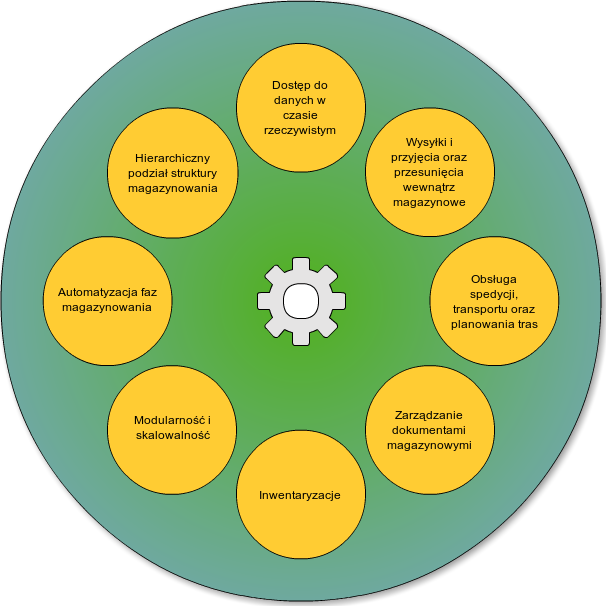
\includegraphics[width=0.95\textwidth]{images/wms_functionality_2}
		\end{center}
		\caption[Funkcjonalność systemu WMS]{
			Funkcje systemu WMS\\
			źródło: opracowanie własne na podstawie \cite{logistyka_w_przedsiebiorstwie}
		}
		\label{fig:c5:wms_basic_functionality}
	\end{figure}
	\subsection{Zarządzanie wieloma magazynami przez jeden interfejs}
		Magazyny w tym ujęciu mogą być zarówno traktowane jako logiczne\footnote{Wydzielone z magazynu fizycznego
		aby ułatwić zarządzanie.} lub fizyczne, a ich liczba nie jest z natury ograniczana. Przykładowo w przedsiębiorstwie
		produkcyjnym można wyróżnić z pewnością co najmniej 2 rodzaje magazynów:
		\begin{itemize}
			\item magazyn wejścia, skład surowców do produkcji;
			\item magazyn wyjścia, skład produktów gotowych.
		\end{itemize}			
		Dzięki możliwości zdefiniowania dowolnej ich liczby oraz struktury, system WMS oddaje do użytku
		pierwszą ze swoich cech, jaką jest \textbf{możliwość dopasowania do potrzeb odbiorcy}.
		Same magazyny, abstrahując od rodzaju\footnote{W tym wypadku chodzi o to, czy o danym magazynie mówimy jako
		o magazynie fizycznym, czy też logicznym}, można następnie dzielić dowolnie na kolejne, coraz to mniejsze 
		jednostki strukturalne.
	\subsection{Obszar magazynowy - jak zarządzać strukturą}	
		\begin{figure}[h]
			\centering
			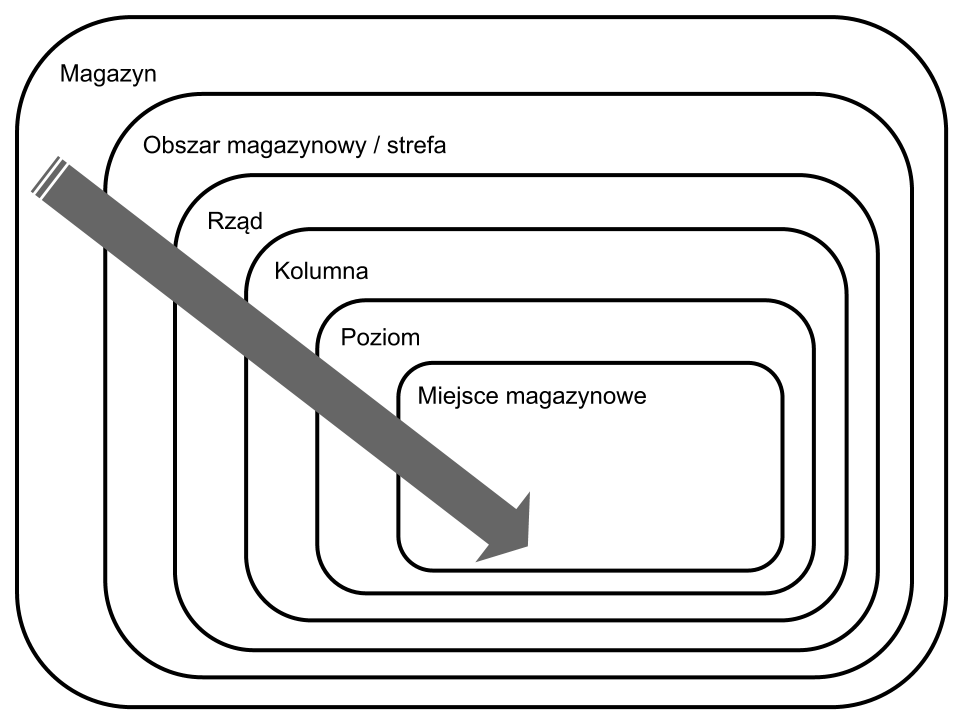
\includegraphics[width=\textwidth]{images/unit_structure}
			\caption[Podstawowa struktura magazyny]{
					Podział struktury magazynowej w wersji podstawowej. \\
					źródło: opracowanie własne
			}
			\label{fig:c5:unit_structure}
		\end{figure}
		Obszary logiczne są odzwierciedleniem podstawowego układu magazynu, na który składają się:
		\textbf{strefy wydań, składowania, kompletacji oraz przyjęć}. Przykładowo można wyróżnić obszary:
		\begin{itemize}
			\item banda załadunkowa, gdzie magazyn wysokiego składu wykonuje zadania automatycznej kompletacji
			zamówienia;
			\item obszar magazynowania blokowego, gdzie składowane są towary nie możliwe do umieszczenia
			na regałach;
			\item bandy rezerwowe, na których system może automatycznie umieścić źle oznakowane bądź bądź
			uszkodzone towary.
		\end{itemize}
		Podobnych przykładów jest z pewnością więcej, ale ich wspólną cechą jest to, że wynikają one z 
		charakterystyki samego magazynu, która to z kolei jest wynikiem procesu wdrożeniowego dostosowanego
		dla konkretnego odbiorcy.\\
		Magazyn nie musi się jednakże dzielić na obszary funkcjonalne. Możliwy jest podział także ze względu
		na charakter składowanych artykułów. Przykładowo w przypadku branży spożywczej niedopuszczalne będzie
		umieszczenie owoców cytrusów w tym samym obszarze składowania, który przeznaczony jest dla 
		warzyw z rodziny czosnkowatych.
	\subsection{Miejsca magazynowe - kolejny poziom układu}
		\begin{figure}[h]
			\centering
			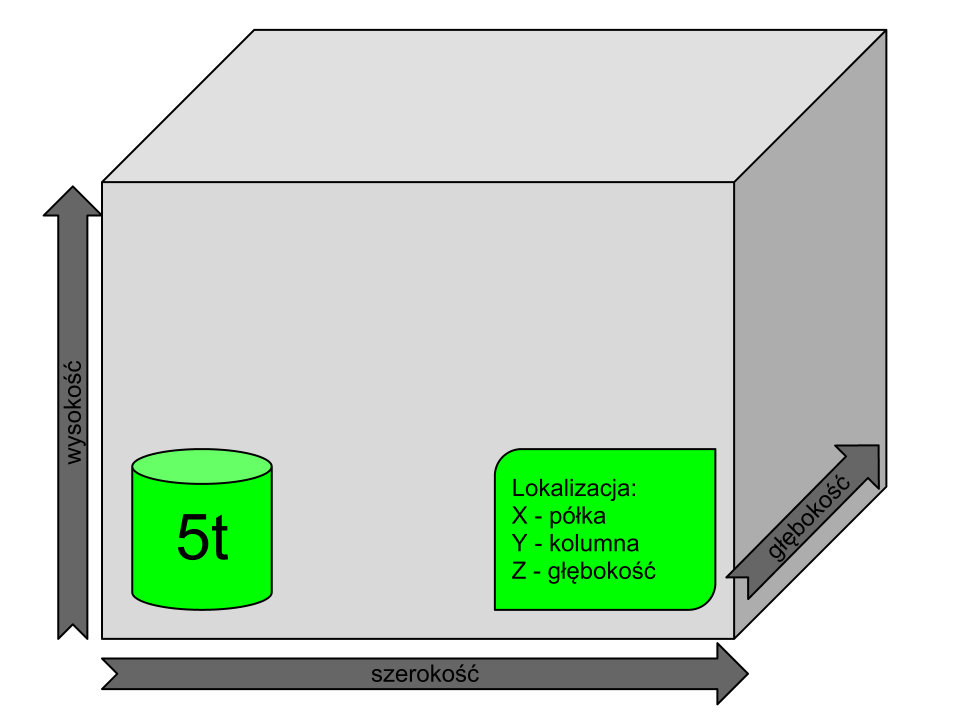
\includegraphics[width=\textwidth]{images/storage_unit_description}
			\caption[Miejsce magazynowe - właściwości fizyczne]{
					Właściwości fizyczne miejsca magazynowego dla magazynu wysokiego składu \\
					źródło: opracowanie własne na podstawie \cite{IDL}
			}
			\label{fig:c5:storage_unit_description}
		\end{figure}
		Zgodnie z rysunkiem \ref{fig:c5:unit_structure}, podstawową jednostką strukturalną jest miejsce magazynowe.
		Również w tym wypadku dobrze zaprojektowany system wspomagania gospodarki magazynowej, daje 
		użytkownikowi końcowemu możliwość takiego skonfigurowania oraz przystosowania swojej aplikacji,
		aby jej parametry odpowiadały rzeczywistym w sposób najbardziej wierny. I tak można więc opisać miejsce 
		magazynowe za pomogą parametrów fizycznych, jak to opisane zostało na rysunku \ref{fig:c5:storage_unit_description},
		oraz parametrów niefizycznych, które odwołują się sposobów identyfikacji danego miejsca 
		w systemie oraz określenia poziomu jego wypełnienia. 
	\subsection{Zawartość magazynu - sposoby eksploracji}
		Systemy klasy WMS pozwalają oczywiście na prowadzenie ewidencji ilościowej i wartościowej całego
		składowanego asortymentu. Prócz tego dostarczają również ważnej funkcjonalności odnoszącej się do cech asortymentu,
		daleko wykraczających poza podstawowe funkcje. Możliwe jest więc uzyskanie w czasie rzeczywistym informacji na temat
		dokładnego położenia konkretnej, \textbf{jednostkowej} pozycji asortymentu w obszarze składowanie. Można 
		ustalić, czy dana partia towaru jest obecnie przemieszczana, np od strefy wejścia do strefy składowania, czy może
		znajduje się tuż przed wejściem do strefy kompletacji. Jest to ważne z punktu widzenia optymalizacji
		wykorzystania przestrzeni magazynowej. \\
		
		\textbf{Algorytmy ABC, XYZ} stanowią najprostszy sposób uzyskania efektu zoptymalizowania rozkładu produktów. I tak
		te dobra, których \textbf{współczynnik rotacji} jest wysoki znajdują się w miejscach magazynowych, zlokalizowanych
		najbliżej strefy kompletacji, a za co tym idzie wydań. Dzięki temu wydanie takiego towaru okazuje się być
		zadaniem łatwiejszy o znacznie skróconym czasie realizacji, co jest zjawiskiem pożądanym z punktu widzenia przedsiębiorstwa,
		mającego w swojej misji punkt traktujący o \textit{terminowości dostaw}. 
			\paragraph{Algorytm ABC} jest metoda wywodzi się od \textit{reguły Pareto}, 
			która odwołuje się do zależności 80\%-20\%. W kontekście składowania towarów 
			w magazynach, można powiedzieć, że 20\% pozycji stanowi 80\% wartości
			wszystkich produktów. Używając analizy ABC można więc dokonać przypisania 
			poszczególnych towarów do poszczególnych grup:
			\begin{itemize}
				\item \textbf{Grupa A} - są to towary najbardziej cenne, których liczebność
				dochodzi do 20\%, ale mające znaczenie większy udział w wartości sięgające
				do 80\%;
				\item \textbf{Grupa B} - grupa środkowa, do której przypisane są te zapasy, których
				udział procentowy w kontekście ilościowym oraz wartościowym waha się między 15\% a 20\%;
				\item \textbf{Grupa C} - grupa o najmniejszym udziale wartościowym, ale o największym udziale
				ilościowym, dochodzącym do 80\%.
			\end{itemize}
			
			\paragraph{Algorytm XYZ} - stanowi odwrotność metody ABC, ponieważ nie odwołuje się
			do struktury zapasów opartej o podejście ilość-wartość. Celem metody XYZ jest podzielenie
			zapasów na grupy, które oddaję strukturę oraz częstość z jaką są one użytkowane. Wyróżnione
			są więc następuje kategorie (grupy):
			\begin{itemize}
				\item \textbf{Grupa X} - materiały o najbardziej regularnym zapotrzebowaniu;
				\item \textbf{Grupa Y} - materiały, na które zapotrzebowanie ma charakter sezony, rosnący
				np. w okresie letnim;
				\item \textbf{Grupa Z} - materiały, na które zapotrzebowanie jest wysoce nieregularne.
			\end{itemize}			 
			
	\subsection{Eksploracja struktury magazynu}
		Nie warto chyba przypominać jak ważne jest wiedzieć, gdzie w danej chwili znajduje się dana pozycja asortymentowa.
		Co ważniejsza, wiedza taka jest tym bardziej wartościowa, im większy jest stopień szczegółowości położenia towaru. 
		Niemniej są to informacje, które są użyteczne z punktu widzenia systemu informatycznego, a dla człowieka mogą
		pozostawać nie do końca czytelna. Dlatego właśnie tak ważne staje się utrzymanie pełnej mapy struktur obszarów
		składowania, dzięki którym to użytkownik końcowy, jest w stanie jednoznacznie wskazać lokalizację pozycji towarowej,
		a następnie może dotrzeć do niej fizycznie. Jednym ze sposobów dostarczenia takiej funkcjonalności jest 
		udostępnienia interfejsu wykorzystującego mapę powierzchni magazynowej w formie drzewiastej, podobnej to 
		struktury katalogów.
		\begin{figure}[H]
			\centering
			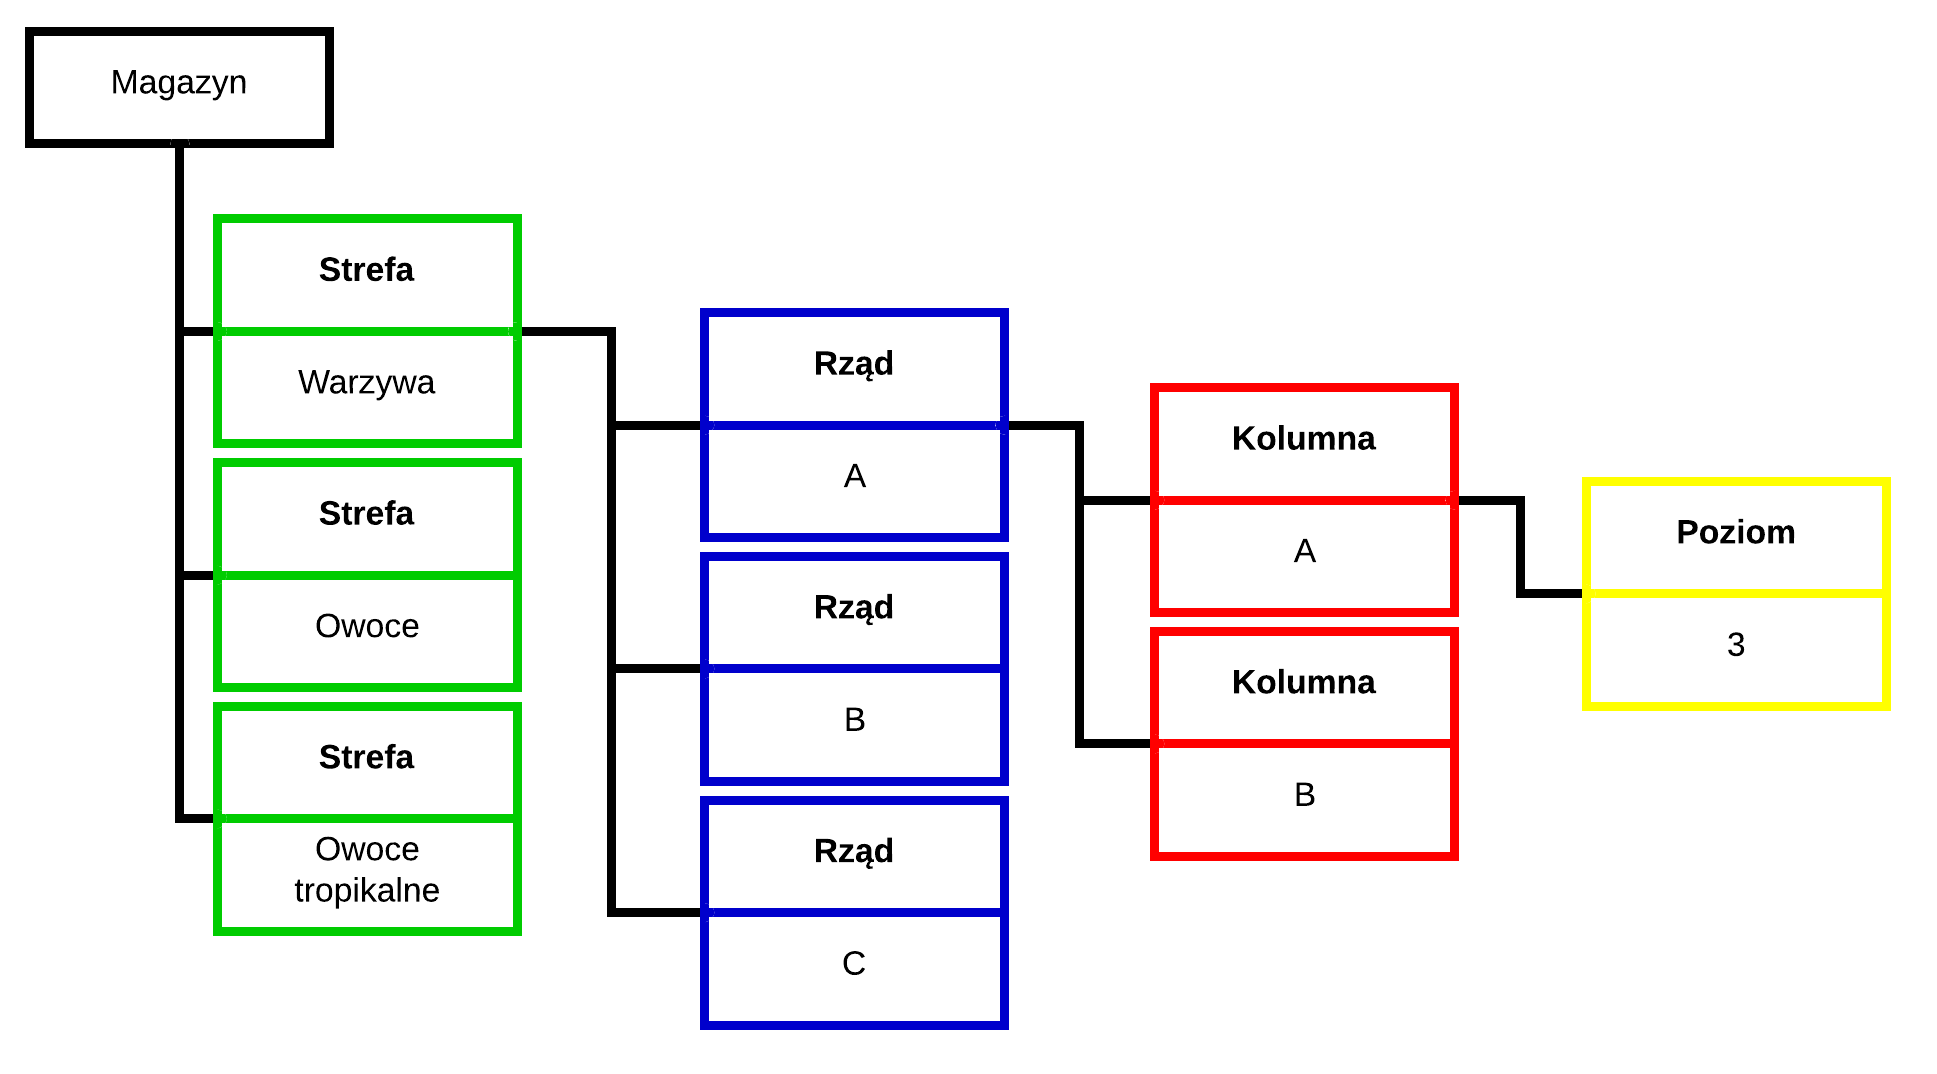
\includegraphics[width=1.1\textwidth]{images/warehouse_tree}
			\caption[Przykładowe drzewo eksploracji magazynu]{
				Drzewo struktury magazynu\\
				źródło: opracowanie własne
			}
		\end{figure}
		W takim drzewie można wyróżnić korzeń, który oznacza konkretny fizyczny magazyn, a kolejne poziomy oznaczają 
		kolejne poziomy szczegółowości opisu położenia jednostek ładunkowych. Jako liście mogą być zaznaczone zarówno
		konkretne produkty, jak i również konkretne miejsca magazynowe. \\
		
		Dodatkowym atutem jest dostarczenie możliwości wyszukiwania informacji poprzez system prostych zapytań, 
		znanych chociażby z przeglądarki Google, która prócz wyszukiwania prostego, pozwala na doprecyzowania
		wyników do: zawierania konkretnych słów kluczowych lub szukania w określonym zakresie witryn. W odniesieniu
		do omawianej klasy systemów, zapytanie mogłoby przyjąć postać: \emph{Pokaż wszystkie paletowe jednostki
		ładunkowe o masie większej niż 2t, znajdujące się w obszarach od 1 do 3}. 
	\subsection{Dokumenty logistyczne jako element niezbędny w zarządzaniu}
		Dokumenty logistyczne albo bardziej dobitnie dokumentacja jest podstawową do prowa\-dzenia odpowiedniej
		ewidencji dynamiki magazynu, do dostępu do danych historycznych, które często stosuje się
		do planowania strategicznego oraz operacyjnego. Najważniejszą być może, ale nie jedyną, grupę dokumentów
		stanowią te, opisujące wydania, przyjęcia, przesunięcia odpowiednio z, do, między i wewnątrz magazynu.
	\subsubsection{Obsługa zamówień oraz zleceń}
		W kontekście tematu zamówień oraz zleceń, będących integralną częścią procesów dotyczących fizycznego
		przemieszczania towarów, materiałów lub produktów w magazynie. Dokumentem właściwym dla zamówień są
		\textbf{wydania magazynowe}, a same dokumenty skierowane są do odbiorcy towarów firmy, będącej właścicielem
		wykupionych powierzchni magazynowych lub całego obiektu. Z drugiej strony działanie obiektu magazynowego
		nie opiera się wyłącznie na wydaniach. Na drugiej stronie szali znaleźć można \textbf{przyjęcia magazynowego},
		dla których dokumentem właściwym są zamówienia skierowane dla dostawców. Jeśli spojrzeć na magazyn ponownie jako
		na element buforujący, równoważący podaż i popyt na rynku, to można spojrzeć na wydania magazynowego jako
		elementy lub synonim popyt, a przyjęcia magazynowe odpowiadają podaży. 
		
		\begin{figure}[H]
			\centering
			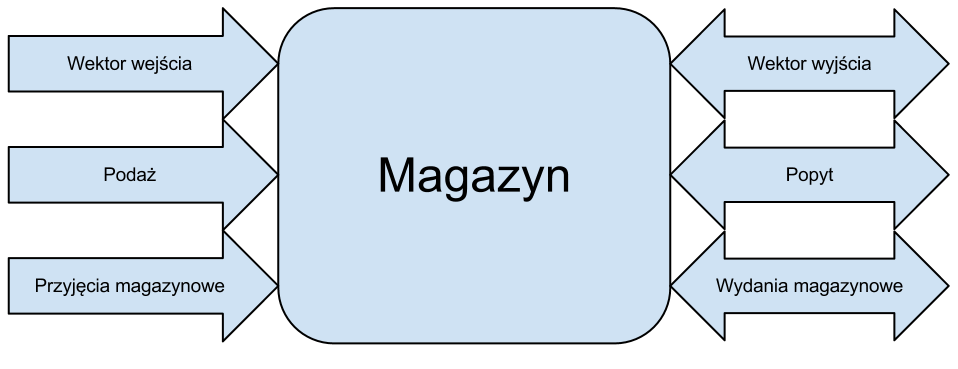
\includegraphics[width=\textwidth]{images/warehouse_buffer}
			\caption[Magazyn jako bufor]{
				Magazyn jako element buforujący podaż i popyt\\
				źródło: opracowanie własne
			}
		\end{figure}
		
		\paragraph{Zamówienia dla dostawców - dokument  - przyjęcie magazynowe} - tworzony jest na podstawie
		aktualnych stanów magazynowych. Czynność, którą jest tutaj zamówienia, może być zautomatyzowana lub wykonana
		przez operatora logistycznego. W obu wypadkach wykorzystuje się raporty generowane przez system WMS i 
		na ich podstawie podejmuje decyzje o zamówieniu \textit{k pozycji} w odpowiednich ilościach. Moduł, obsługujący
		wektor wejścia, jest w wielu przypadkach powiązany lub wykorzystuje algorytmy właściwe dla \textbf{MRPI}. 
		Korzyścią jest więc składaniach zamówień tylko na te produkty i tylko w takich ilościach, jakie są faktycznie wymagane.
		Co ważniejsze moment, w których dokument jest generowany i wysyłany do dostawców, jest wybrany precyzyjnie na
		podstawie dynamiki i struktury zamówień od klientów.
			\subparagraph{Potwierdzenie dokumentów wydania} jest czynnością skojarzoną z \textbf{rezerwacją towarów},
			jednakże to właśnie zastrzeżenie odpowiednich pozycji (we właściwych ilościach) ma pierwszeństwo. 
			Rezerwacja towarów stanowi formalne zabezpieczenie, które uniemożliwia omyłkowe wydania 
			pozycji przeznaczonych dla danego klienta. Zarezerwowane towary zostają zablokowane i nie mogą 
			zostać wykorzystane.
			Potwierdzenie dokumentów wydania jest jedną z form zwolnienia tej blokady. Pozycje, które zostały
			wcześniej zarezerwowane, zostają usunięte ze stanów magazynowych i opuszczają magazyn, zarówno
			system jak i fizyczny budynek. Drugą z opcji, jest sytuacja, kiedy należy wycofać pewne 
			pozycje, ponieważ klient odmówił ich przyjęcia.  
		\paragraph{Zamówienia od klientów -  dokument  - wydania magazynowe} - tworzony jest na podstawie zapotrzebowania
		zgłoszonego przez klienta oraz jego danych. Obie informacja są wystarczającą podstawą do skompletowania
		i fizycznej wysyłki. 
		
		W obu wypadkach ważne jest, że każdy wygenerowany dokument, każde zgłoszone żądania kompletacji, alokacji
		jest rejestrowane i stanowi podstawę do optymalizacji i lepszego zarządzania wektorami wejścia i wyjścia. 
	\subsection{Rezerwacja towarów}
		Działanie, które polega na wczesnym zarezerwowaniu grupy towarów, niekoniecznie jeszcze skompletowanych,
		do wysyłki do konkretnego odbiorcy. Rezerwacja jest w tym wypadku \textbf{wyłączna}, a wykorzystane
		pozycje nie podglądają użyciu w jakikolwiek inny sposób. Jest to dosyć przydatna funkcja systemy magazynującego.\\
		
		Hipotetyczna sytuacja zakłada prawie natychmiastowe przekazania wyprodukowanych jednostek do strefy kompletacji,
		celem wydania ich klientowi. Niestety towar ma okres przestojowy, który musi odstać w strefie składowania, 
		zanim będzie można go przekazać dalej. Chcemy uzyskać pewność, że wymagane pozycje będą gotowe
		dla wybranego klienta, któremu zależy na szybkiej realizacji. Na wszystkie towary objęte zamówienie nakładana
		jest rezerwacja i są one jednocześnie umieszczane na miejscach odkładczych, które zlokalizowane są najbliżej
		strefie wyjścia. Po upłynięciu okresy odstania, system WMS automatycznie wydaje towar do strefy składowania.\\
		Inną teoretyczną sytuacją byłaby taka, w której zamówienia nadeszło by z terminem realizacji natychmiastowej, w ciągu
		zaledwie 12h. Klient jest jednym jednym z największych odbiorców, więc użycie rezerwacji wydaje się właściwe. \\
		
		Niemniej problem rezerwacji towarów nie jest tak oczywisty, jak się wydaje. Nie można nadużywać tego rozwiązania,
		aby promować odbiorców, charakteryzujących się częstymi zamówienia i lepszą strukturą płatności. Dla przedsiębiorstwa
		jutra ważne jest nie tyle sprostanie wymaganiom kilku, ale sukcesywne budowanie swojej marki w szerokim gronie
		odbiorców. 
	\subsection{Automatyczne planowanie fizycznych wysyłek}
		Ten moduł oprogramowania WMS ma jeden cel - \emph{dokonać automatycznego utworzenia jednej fizycznej wysyłki}.
		Planowanie takiej dostawy odbywa się na z góry określonych warunkach. Określona zostaje jednostka ładunkowa, na
		której mają zostać umieszczone produkty, a także nadrzędne kryterium grupowania. I tak na samochodzie dostawczym
		znajdą się towary ustawione zgodnie z kolejnością wyładowywania. \\
		
		Podczas planowania przesyłka może znaleźć się w trzech stanach:
		\begin{enumerate}
			\item \textbf{Edycja przesyłki} - w danym momencie przesyłka znajduje się wciąż na etapie planowania, dokładane
			są kolejne pozycje asortymentowe;
			\item \textbf{Edycja przesyłki} - następuje bezpośrednio po zakończeniu poprzedniego etapu. \linebreak
			W tym punkcie nacisk nastąpiło już wystosowanie żądania rozpoczęcia kompletacji;
			\item \textbf{Dostarczona} - ten stan wysyłka otrzymuje, jeśli została ona zrealizowana.
		\end{enumerate}

		\subsubsection{Problem efektywnej realizacji kompletacji}
			Realizacja kompletacji w systemie WMS polega na pobraniu wszystkich pozycji znajdujących się na wydaniach
			magazynowych, pobraniu ich z odpowiednich, często wcześniej wskazanych, miejsc składowania i transporcie
			do strefy kompletacji. W tym miejscu pojawia się najwięcej różnicy, odnoszących się do sposobu radzenia
			sobie z tym problem, a rozwiązanie zależy silnie od stopnia wdrożenia. Jeśli procesy magazynowe
			w przedsiębiorstwie są wspierane przez techniki automatycznej identyfikacji\footnote{Automatyczna
			identyfikacja może być zarówno oparta o skanowanie kodów kreskowych lub o technikę RFID}. Im większy stopień
			automatyzacji oraz szczegółowości opisu pozycji asortymentowych, tym mniejsza prawdopodobieństwo 
			wystąpienia pomyłek i strat magazynowych.		
		
	\subsection{Dostawy do magazynu}
		Dostawy do magazynu są zbiorem operacji związanych z czynnościami fizycznymi oraz systemowymi
		przyjęcia zamówienia na stan magazynowy. Od strony fizycznej obejmują kontrole jakościowe
		oraz ilościowe, a od strony systemu WMS automatyczne przydzielenie miejsc odkładczych,
		zgodnie z przyjętymi regułami oraz wprowadzenie danych do systemu. 	
			\paragraph{Dostawy zewnętrzne} stanowią podzbiór dostaw i odnoszą się do wszystkich operacji,
			gdzie zamówione towary pochodzą z zewnątrz. Obsługa tego typu sytuacji obejmuje kontrole
			ilościowe i jakościowe oraz rozłożenie towaru w magazynie. Alokacja odbywa się automatycznie
			na podstawie przyjętej strategii. Warto w tym miejscu wspomnieć, że dostawa zewnętrzna może,
			ale nie musi, wymagać przepakowania dostarczonych towarów lub umiesz\-czenia ich na nośniku,
			którego składowania jest możliwe w danym magazynie. Oczekiwanym wynikiem tej operacji jest:
			\begin{enumerate}
				\item uaktualnienie stanów magazynowych;
				\item zarejestrowania dostawy.
			\end{enumerate}\pagebreak			
			\paragraph{Dostawy wewnętrzne} odnoszą się do przesunięć wewnątrz magazynowych oraz w większym
			stopniu do dostaw z produkcji. Nie występuje problem z nośnikiem produktów, ponieważ 
			opuszczają one linie produkcyjną w stanie, w którym można je bezproblemowo składować. Jednostki
			logistyczne są etykietowane, co umożliwia ich późniejszą identyfikacją. 
			Oczekiwanym wynikiem tej dostawy wewnętrznej jest:
			\begin{enumerate}
				\item zwiększenie stanów magazynowych;
				\item umieszczenie odpowiednich etykiet.
			\end{enumerate}		 						
	\subsection{Wysyłki z magazynu}
		Wszystkie operacja odnoszące się do opuszczania przez produktu systemu magazynowego odnoszą się do zjawiska
		przeciwnego do podaży - popytu. W odniesieniu do klasy systemów WMS, najczęściej mówi się o automatycznym
		planowaniu wysyłki, jako reakcji na zamówienie klienta. Odpowiednie algorytmy wiedzą, gdzie znajdują
		się konkretne pozycje i są w stanie przekierować je do strefy kompletacji, dla danego zamówienia, w ilości
		zgodnej z podaną na dokumencie. Dodatkowym autem takiego podejścia, jest to, że systemy wspomagające
		zarządzania magazynem bardzo często posiadają wsparcia dla planowania tras. Taka możliwość wpływa dodatnio
		na operacje planowania kompletacji, gdyż algorytm obsługujący tę operację, jest w stanie tak rozłożyć
		zamówione produkty, aby odpowiadały trasom dostaw, w sposób najbardziej optymalny. 		
			\paragraph{Realizacja kompletacji} polega na wygenerowaniu nośników do kompletacji, o typie zgodnym z profilem
			zamówionych produktów, oraz pobraniu odpowiednich materiałów lub produktów z wyznaczonych miejsc
			składowania. W tym momencie ważna staje się charakterystyka działalności przedsiębiorstwa, które jest 
			właścicielem powierzchni magazynowych. Zawartość nośnika może być bowiem jednorodna (firma produkująca
			papier), jak i niejednorodna. Niemniej po zebraniu wszystkich wskazanych produktów, następuje kontrola
			ilościowa.			
	\subsection{Autonomiczność systemów klasy WMS}
		Bardzo często dzieje się tak, że system wspomagający magazynowanie nie jest jednostką samodzielną, ale 
		stanowi część większego \textbf{ZSI} - \textit{Zintegrowanego Systemu Informatycznego}. Między tymi
		dwoma rozwiązaniami istnieje istotna różnica, która jest równocześnie powodem ich koegzystencji.
			\paragraph{Zarządzanie zapasami} przez ZSI odnosi się do ich ilościowej, jak i jakościowej natury. Z
			drugiej strony WMS zarządza nimi w kontekście ich fizycznej lokalizacji i stanów magazynowych. Co
			ważniejsze te dwa podejście uzupełniają się dając pełny obraz koordynatorom logistycznym na temat
			struktury zapasów itp. 
			\paragraph{Autonomiczne operacje} systemu WMS odnoszą się do jego możliwości monitorowania ruchów
			jednostek logistycznych w całym systemie już do momentu, kiedy się w nim znalazły, aż do momentu,
			kiedy opuszczają magazyn. Operatorzy logistyczni są więc wypo\-sażeni w funkcje, które pozwalają
			im przenieść określoną ilość wybranych materiałów z jednego miejsca w drugie, ale nie tylko.
			\begin{figure}[H]
				\centering
				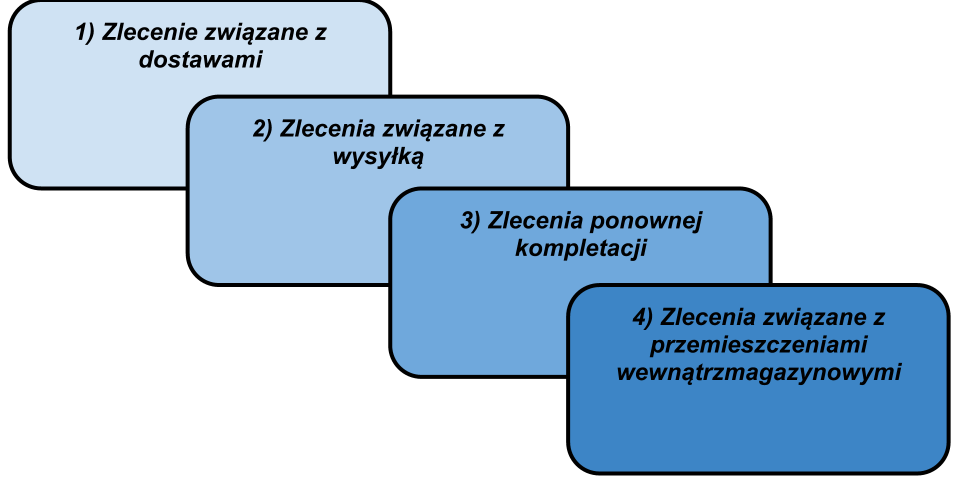
\includegraphics[width=\textwidth]{images/transport_ops}
				\caption[Operacja transportowe w magazynach]{
					Typy operacji transportowych w magazynach\\
					źródło: opracowanie własne na podstawie \cite{IDL}
				}
			\end{figure}